\documentclass[tikz,border=10pt]{standalone}
\usepackage{tikz}
\usetikzlibrary{automata, positioning, arrows.meta, bending}
\usetikzlibrary{calc}

\begin{document}
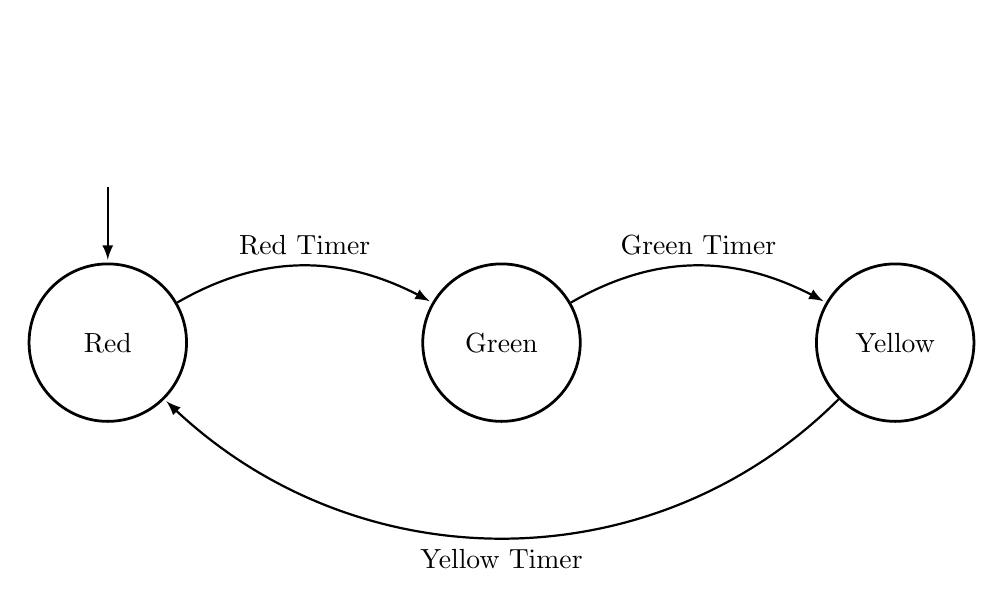
\begin{tikzpicture}[shorten >=1pt,node distance=5cm,on grid,auto,line width=1pt, every edge/.style={draw, -latex, thick},state/.style={circle, draw, minimum size=2cm}]
   \node[state] (q_1) {Red};
   \node[state] (q_2) [right=of q_1] {Green};
   \node[state] (q_3) [right=of q_2] {Yellow};
   \node[state,draw=none] (q_4) [above = 3cm of q_1] {};
   
   \path[->]
   (q_1) edge[bend left] node {Red Timer} (q_2)
   (q_2) edge[bend left] node {Green Timer} (q_3)
   (q_3) edge[bend left=45] node {Yellow Timer} (q_1)
   (q_4) edge node {} (q_1);
\end{tikzpicture}
\end{document}
